\chapter{Digit classifier}\label{ch:digitclass}
Taking advantage of the \glspl{cnn} impressive performance in classification tasks, we have built a \emph{real-time digit classifier}. Its core elements are:
\begin{itemize}
	\item A \emph{Keras model} (see Section~\ref{subsec:models}), which classifies the images.
	\item A \emph{JdeRobot component}, which acquires and processes the images from a video stream and integrates a Keras model to classify them. The images and the classification results are displayed within a \gls{gui}.
\end{itemize}

\section{Understanding the Keras model}\label{sec:understanding}
Understanding how Keras models work is a key factor in the development of this project. For this purpose, an adapted version of an example provided by Keras\footnote{\url{https://git.io/vH0qw}} will be analyzed in the following sections. In this example, a \gls{cnn} is trained and tested with the \emph{\gls{mnist} database} of handwritten digits (see Section~\ref{sec:datasets}).

\subsection{Adapting data}\label{subsec:adaptdata}
First of all, the input data have to be loaded and adapted. Keras library contains a module named \textit{datasets} from which a variety of databases can be imported, including \gls{mnist}. The \gls{mnist} database can be loaded calling the \textit{mnist.load\_data()} method. It returns, as \emph{Numpy arrays}, the images and labels from both training and test datasets, as it is shown in the code below, which also displays the first sample of the \gls{mnist} training dataset (see Figure~\ref{fig:firstsample}).
\begin{lstlisting}
(x_train, y_train), (x_test, y_test) = mnist.load_data()

cv2.imshow('First sample',x_train[0])
cv2.waitKey(5000)
cv2.destroyWindow('First sample')

print ('Original input images data shape: ', x_train.shape) 
\end{lstlisting}

That code also prints the shape of the dataset:
\begin{Verbatim}[frame=single]
Original input images data shape:  (60000, 28, 28)
\end{Verbatim}

\begin{figure}
	\centering
	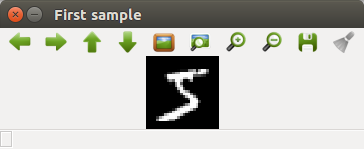
\includegraphics[width=0.7\linewidth, keepaspectratio]{figures/first_sample.png}
	\caption{First sample of the MNIST database.}
	\label{fig:firstsample}
\end{figure}

According to that, the training dataset includes~60000~images, each one containing~28x28~pixels. In order to feed the Keras model, the number of channels of the samples have to be explicitly declared, so the dataset must be \emph{reshaped}. In this case, the samples are \emph{grayscale images}, which implies that the number of channels is equal to 1. For instance, if they had been RGB images, the number of channels would have been equal to 3. As data are stored in Numpy arrays, it can be reshaped using the \textit{.reshape()} method. The order in which dimensions must be declared depends on the \textit{.image\_dim\_ordering()} parameter of the Keras \textit{backend}, as it is shown in the following code.
\begin{lstlisting}
img_rows, img_cols = 28, 28
...
if backend.image_dim_ordering() == 'th':
	# reshapes 3D data provided (nb_samples, width, height) into 4D
	# (nb_samples, nb_features, width, height) 
	x_train = x_train.reshape (x_train.shape[0], 1, img_rows, img_cols)
	x_test = x_test.reshape (x_test.shape[0], 1, img_rows, img_cols)
	input_shape = (1,img_rows,img_cols)
	print ('Input images data reshaped: ', (x_train.shape))
	print ('--------------------------------------------------------------')
else:
	# reshapes 3D data provided (nb_samples, width, height) into 4D
	# (nb_samples, nb_features, width, height) 
	x_train = x_train.reshape(x_train.shape[0], img_rows, img_cols, 1)
	x_test = x_test.reshape(x_test.shape[0], img_rows, img_cols, 1)
	input_shape = (img_rows, img_cols, 1)
	print ('Input images data reshaped: ', (x_train.shape))
	print ('--------------------------------------------------------------')
\end{lstlisting}

In this case, the training dataset gets reshaped as follows:
\begin{Verbatim}[frame=single]
Input images data reshaped:  (60000, 28, 28, 1)
\end{Verbatim}

The last step to get the input images ready is to convert \emph{data type} from \textit{uint8} to \textit{float32} and normalize pixel values to $[0,1]$ range:
\begin{lstlisting}
print('Input images type: ',x_train.dtype)
x_train = x_train.astype('float32')
x_test = x_test.astype('float32')
print('New input images type: ',x_train.dtype)
print ('-----------------------------------------------------------------')
x_train /= 255
x_test /= 255
\end{lstlisting}

Regarding the \emph{labels}, they are originally shaped as an array in which each element is an integer in the range $[0, 9]$, i.e. each element contains the digit that corresponds to a certain sample. In order to feed the Keras model, the labels have to be reshaped into an array in which each element must be a \emph{probability distribution}. For example, if the element of the original array is 2, in the reshaped array it will be $[0, 0, 1, 0, 0, 0, 0, 0, 0, 0]$. This conversion is achieved using the Keras built-in method \emph{\textit{np\_utils.to\_categorical()}}:
\begin{lstlisting}
nb_classes = 10
...
print ('First 10 class labels: ', (y_train[:10]))
print ('Original class label data shape: ', (y_train.shape))
# converts class vector (integers from 0 to nb_classes) to class matrix
# (nb_samples, nb_classes)
y_train = np_utils.to_categorical(y_train, nb_classes)
y_test = np_utils.to_categorical(y_test, nb_classes)
print ('Class label data reshaped: ', (y_train.shape))
print ('-----------------------------------------------------------------')
\end{lstlisting}

That code prints:
\begin{Verbatim}[frame=single]
First 10 class labels:  [5 0 4 1 9 2 1 3 1 4]
Original class label data shape:  (60000,)
Class label data reshaped:  (60000, 10)
\end{Verbatim}

\subsection{Model architecture}
Once the data are ready, the \gls{cnn} architecture must be defined. In this example, a \emph{sequential model} (see Section~\ref{subsec:models}) is enough for solving the classification task and it is declared as follows:
\begin{lstlisting}
model = Sequential()
\end{lstlisting}

The next step is to add the corresponding layers. The core layers of a \gls{cnn}, as treated by Keras, have been already defined in Section~\ref{subsec:layers}. The following code performs the addition of the layers to the model.
\begin{lstlisting}
nb_filters = 32
kernel_size = (3, 3)
pool_size = (2, 2)
...
# convolutional layer
model.add(Convolution2D(nb_filters, kernel_size[0], kernel_size[1],
                          border_mode='valid', input_shape=input_shape, 
                          activation='relu'))
# convolutional layer
model.add(Convolution2D(nb_filters, kernel_size[0], kernel_size[1],
                          activation='relu'))
# pooling layer
model.add(MaxPooling2D(pool_size=pool_size))
# dropout layer
model.add(Dropout(0.25))
# flattening the weights (making them 1D) to enter fully connected layer
model.add(Flatten())
# fully connected layer
model.add(Dense(128, activation='relu'))
# dropout layer to prevent overfitting
model.add(Dropout(0.5))
# output layer
model.add(Dense(nb_classes, activation='softmax'))
\end{lstlisting}

As defined by the code above, the model is formed by the following layers:
\begin{itemize}
	\item A \emph{2D convolutional layer} with~32~filters whose size is~3x3x1.
	\begin{itemize}
		\item Since this is the first layer of the model, the \emph{\textit{input\_shape}} argument must be provided. In this case, the input shape is~28x28x1. 
		\item As \textit{valid} mode is set, \emph{no padding} is applied and the output dimension will be reduced. 
		\item \emph{\gls{relu} activation function} (see Equation~\ref{eq:relu}) introduces non-linearity into the network. If the activation functions were linear, the whole stack of layers could be reduced to a single layer, losing much of the ability to learn different levels of features.
		\item This layer outputs~32~activation maps with size~26x26.
	\end{itemize}
	
	\item Another \emph{convolutional layer} with the same arguments:~32~filters, no padding and \gls{relu} as activation function.
	\begin{itemize}
		\item Increasing the number of convolutional layers allows the \gls{cnn} to learn \emph{more complex features}. 
		\item As the depth of its input is~32~(one channel per activation map), the size of the filters will be~3x3x32. 
		\item This layer outputs~32~activation maps with size~24x24.
	\end{itemize}
	
	\item A \emph{2D MaxPooling layer} with a \textit{pool\_size} of~2x2.
	\begin{itemize}
		\item This layer outputs the~32~activation maps generated by the previous layer, but \emph{\textit{downsampled}} by a factor of~2, resulting in maps with size~12x12.
	\end{itemize}
	
	\item A \emph{dropout layer} to prevent overfitting. 
	\begin{itemize}
		\item The fraction of random units that are going to be \emph{\textit{swicthed-off}} is~0.25.
		\item This layer preserves the size and the shape of its input.
	\end{itemize} 
	
	\item A \emph{flatten layer} that turns the matrices of weights that it receives at its input into a vector that can be fed to the fully-connected layer.
	\item A fully-connected or \emph{dense layer}.
	\begin{itemize}
		\item This layer contains~128~neurons that will output an array of~128~values.
		\item Once more, the \emph{\gls{relu} activation function} is applied.
	\end{itemize} 
	
	\item A \emph{dropout layer} with a~0.5~fraction.
	
	\item Finally, the \emph{output layer} is another \emph{dense layer} which contains as many neurons as classes, in this example,~10. 
	\begin{itemize}
		\item In order to output a \emph{probability distribution} of the predicted classes, the activation function will be \emph{softmax} (Equation~\ref{eq:SoftMax}).
	\end{itemize}
\end{itemize}

The resulting architecture and data shape after every layer are shown in Figure~\ref{fig:model}.

\begin{figure}
	\centering
	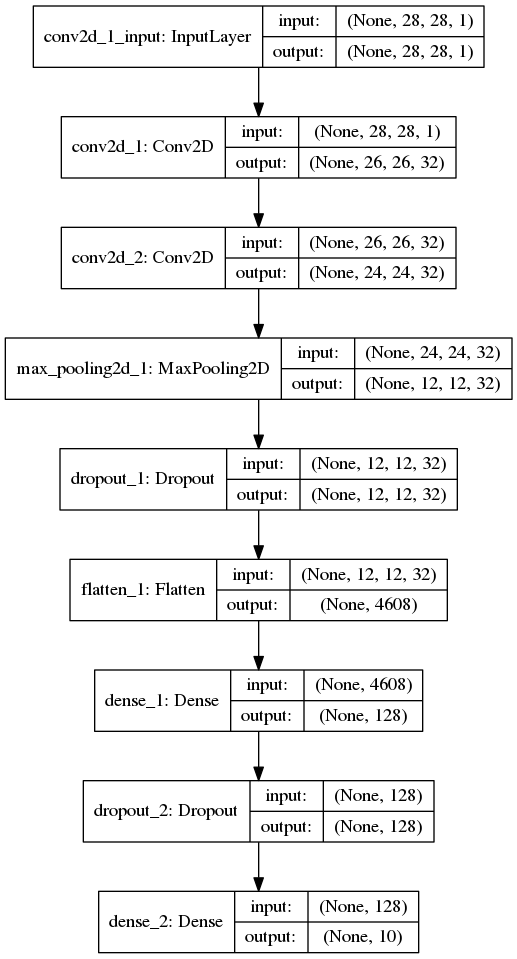
\includegraphics[width=0.6\linewidth, keepaspectratio]{figures/model.png}
	\caption{Diagram of a Keras sequential model.}
	\label{fig:model}
\end{figure}

\subsection{Compiling the model}
After declaring the model and defining its architecture, the \emph{learning process} must be set through the  \textit{.compile()} method. The arguments required to set this process are defined in Section~\ref{subsec:models}. The code can be seen in the next frame:
\begin{lstlisting}
model.compile(loss='categorical_crossentropy', optimizer='adadelta', 
               metrics=['accuracy'])
\end{lstlisting}

In this example, the loss function that is computed after every batch is the \emph{categorical cross-entropy} (see Equation~\ref{eq:categorical_crossentropy}) and the optimizer that updates the weights of the \gls{cnn} in order to minimize that loss function is \emph{ADADELTA}. Additionally, the \emph{accuracy} is also computed to monitor the \gls{cnn} performance during training.

\subsection{Training the model}
The \gls{cnn} is trained thanks to the \textit{.fit()} method, which has been already described in Section~\ref{subsec:models}. The usage of that method can be seen in the code below.
\begin{lstlisting}
nb_epoch = 12
batch_size = 128
...
model.fit(x_train, y_train, batch_size=batch_size, nb_epoch=nb_epoch,
           verbose=1, validation_data=(x_test, y_test))
\end{lstlisting}

The model will be trained for~12~\emph{epochs} and the \emph{batch size}, i.e. the number of samples that pass through the \gls{cnn} before updating the weights, is~128. The test dataset is used here as \emph{validation data}, for which the log loss and the accuracy will be computed after every epoch just for \emph{monitoring purposes}. During training time, Keras prints the results after every batch and epoch as follows:
\begin{Verbatim}[frame=single]
Train on 60000 samples, validate on 10000 samples
Epoch 1/12
128/60000 [....................] - ETA: 350s - loss: 2.3223 - acc: 0.1016
256/60000 [....................] - ETA: 312s - loss: 2.3073 - acc: 0.1094
...
59776/60000 [==================>.] - ETA: 1s - loss: 0.0455 - acc: 0.9871
59904/60000 [==================>.] - ETA: 0s - loss: 0.0455 - acc: 0.9871
60000/60000 [====================] - 407s - loss: 0.0455 - acc: 0.9871 - 
val_loss: 0.0306 - val_acc: 0.9891
\end{Verbatim}

\subsection{Testing the model}
Once the model is trained, its weights, architecture and learning configuration can be stored in an \emph{\gls{hdf5} file} (see Section~\ref{sec:hdf}). Besides that, in order to see the performance of the \gls{cnn}, the \textit{.evaluate()} method takes the test dataset and computes the \emph{log loss} and the \emph{accuracy}, as it is shown in the following code:
\begin{lstlisting}
model.save('MNIST_net.h5')

score = model.evaluate(x_test, y_test, verbose=0)
print('Test score:', score[0])
print('Test accuracy:', score[1])
\end{lstlisting}
These are the results obtained with this example (\textit{Test score} refers to loss):
\begin{Verbatim}[frame=single]
Test score: 0.0306129640532
Test accuracy: 0.9891
\end{Verbatim}

\section{JdeRobot component}\label{sec:component}
Once the \gls{cnn} has been trained and the resultant model is saved, the next milestone is to integrate it into a JdeRobot component that must be able to acquire images from a video stream, apply the necessary preprocessing and display the predictions obtained from them. That component is \emph{\textit{digitclassifier.py}} and it is based on Nuria Oyaga's code\footnote{\url{https://git.io/vH0qD}}. It relies on \textit{Camera} and \textit{\gls{gui}} classes. Figure~\ref{fig:digitclass} shows the program running.

\begin{figure}
	\centering
	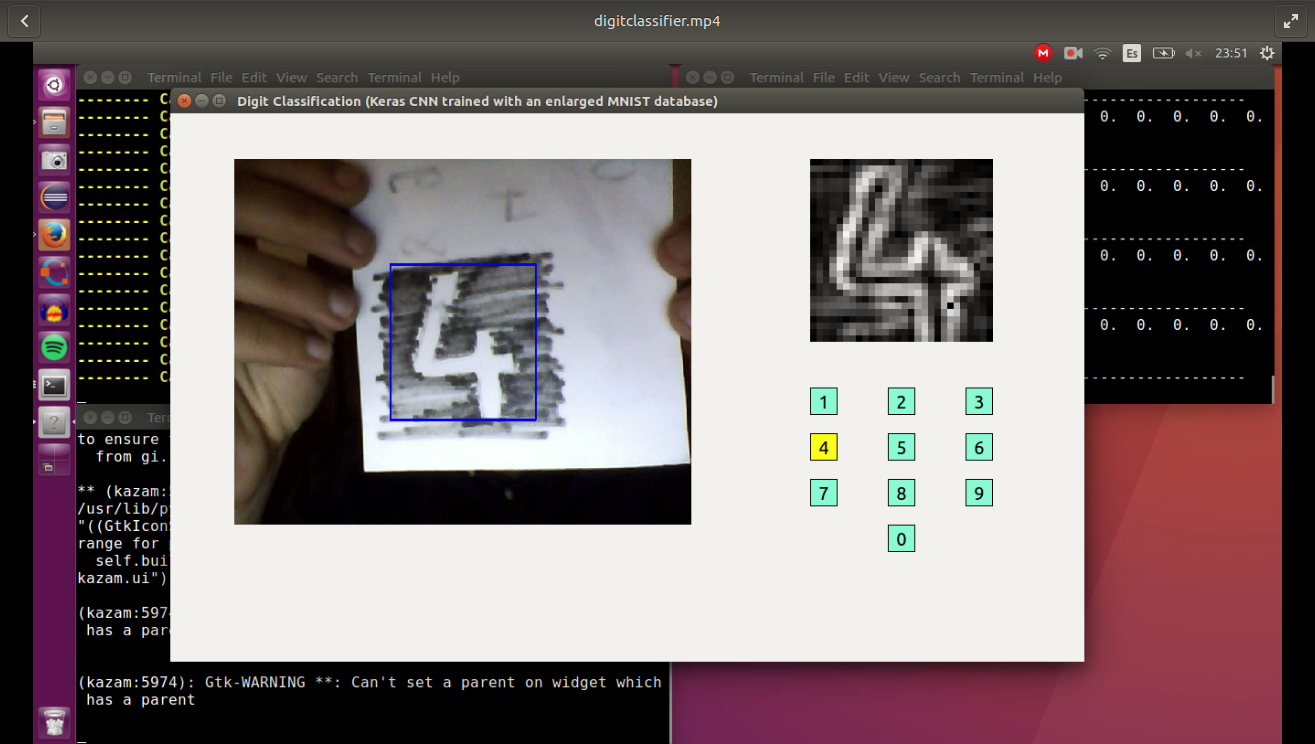
\includegraphics[width=1\linewidth, keepaspectratio]{figures/digitclass.png}
	\caption{Example of \textit{digitclassifier.py} execution.}
	\label{fig:digitclass}
\end{figure}

\subsection{Design}
Before analyzing in detail the internals of the digit classifier component, its design will be described. For this purpose, the \emph{block diagrams} shown in Figure~\ref{fig:dia} have been built.

Figure~\ref{fig:dia}(a) shows a \emph{high-level diagram} of the process followed from the video source to the predicted digit. The images captured with the camera are received by the \emph{cameraserver} driver. Then, the digit classifier component communicates with this driver and get the images. Finally, a prediction is made. Optionally, if the images are captured with a smartphone camera, DroidCam can receive those images and create a camera device that can communicate with the \emph{cameraserver} driver.

In Figure~\ref{fig:dia}(b), the  \emph{internals of the digit classifier component} are shown. The main program (\emph{digitclassifier.py}) starts two threads, \textit{ThreadCamera} and \textit{ThreadGUI}. These threads update \textit{GUI} and \textit{Camera} classes concurrently. \textit{Camera} class communicates with \textit{cameraserver} to get the images, which are then preprocessed. The preprocessed image is fed to the Keras model and a prediction is made. Original and preprocessed images, as well as the predicted digits are passed to the \textit{GUI} class, which displays all of them in the screen.
\begin{figure}
	\begin{subfigure}{1\textwidth}
		\centering
		\includegraphics[width=0.8\linewidth]{figures/diagram_black.png}
		\caption{}
	\end{subfigure}
	\begin{subfigure}{1\textwidth}
		\centering
		\includegraphics[width=0.8\linewidth]{figures/diagram_transparent.png}
		\caption{}
	\end{subfigure}
	\caption{Digit classifier design: (a) high-level; (b) lower-level.}
	\label{fig:dia}
\end{figure}

\subsection{\textit{Camera} class}
\emph{\textit{Camera} class} is responsible for getting the images, transforming them into a suitable input for the Keras model and returning the classification results.

\begin{itemize}
	\item \textbf{Acquisition}. The images are served by the JdeRobot component \emph{\textit{cameraserver}} (see Section~\ref{sec:jderobot}). Depending on how its configuration file (\textit{cameraserver.cfg}) has been set, the images can come from different kinds of video streams. Connection with \emph{webcams} and \emph{video files} is straightforward: the URI property in the configuration file must be changed to the number of device or the path of the video, as it is shown in the code below.
	\begin{lstlisting}[frame=single]
	#0 corresponds to /dev/video0, 1 to /dev/video1, and so on...
	#CameraSrv.Camera.0.Uri=1                                # webcam
	CameraSrv.Camera.0.Uri=/home/dpascualhe/video.mp4        # video file
	\end{lstlisting}
	
	In order to establish a connection with smartphone cameras, the \emph{DroidCam application} for Android has been used (see Section~\ref{sec:droidcam}). As this application turns the video stream provided by the smartphone into a \emph{v4l2\footnote{\url{https://www.linuxtv.org/wiki/index.php/Main_Page}} device driver}, the video stream will be listed as another webcam and the number of device must be set in the \textit{cameraserver} configuration file.
	
	Besides that, the \emph{address} at which the video is being served by the \textit{cameraserver} component must be provided to the \textit{Camera} class through another configuration file: \emph{\textit{digitclassifier.cfg}}.
	
	\item \textbf{Preprocessing}. As the images can be captured with different devices, the \textit{digitclassifier.py} component must apply some preprocessing that mitigates the differences between video streams and that makes the images suitable for the Keras model. The following \emph{transformations} are applied before classification:
	\begin{enumerate}
		\item Images are \emph{cropped} into~80x80~pixels images. The \emph{\gls{roi}} from which cropped images are extracted is draw over the original image, making it easier to aim at digits with the camera.
		\item Color doesn't provide any useful information about digits and \gls{mnist} database is formed by \emph{grayscale images}. For this reason, the images captured with the component are converted into grayscale images as well. 
		\item A \emph{Gaussian filtering} is applied in order to reduce image \emph{noise}. When using this operator, the \emph{kernel size} and the \emph{standard deviation} $\sigma$ in $x$ and $y$ should be specified~\cite{itseez2014theopencv}. In this case, the kernel size will be~5x5~and the standard deviation is automatically calculated depending on that size. The 2D Gaussian filter, as defined in~\cite{sonka1999image}, is given by:
		\begin{equation}
		G(x,y)=\exp(-\frac{x^2+y^2}{2\sigma^2})
		\end{equation}
		\item After reducing noise, the image is \emph{resized} to fit the Keras \emph{model input}. The new size is~28x28~pixels, like \gls{mnist} samples.
		\item Last step is obtaining the \emph{gradient of the images}. Working with this kind of images instead of the original ones allows the application to deal with different light and color conditions. The chosen algorithm for this task is \emph{Sobel filter} (Equation~\ref{eq:sobel}). This will be deeply discussed in Section~\ref{subsec:edge}.
	\end{enumerate}
	
	The following code applies the transformations mentioned above:
\begin{lstlisting}[frame=single]
def trasformImage(self, im):
''' Transforms the image into a 28x28 pixel grayscale image and
applies a sobel filter (both x and y directions).
''' 
	im_crop = im [140:340, 220:420]
	im_gray = cv2.cvtColor(im_crop, cv2.COLOR_BGR2GRAY)
	im_blur = cv2.GaussianBlur(im_gray, (5, 5), 0) # Noise reduction.
	
	im_res = cv2.resize(im_blur, (28, 28))
	
	# Edge extraction.
	im_sobel_x = cv2.Sobel(im_res, cv2.CV_32F, 1, 0, ksize=5)
	im_sobel_y = cv2.Sobel(im_res, cv2.CV_32F, 0, 1, ksize=5)
	im_edges = cv2.add(abs(im_sobel_x), abs(im_sobel_y))
	im_edges = cv2.normalize(im_edges, None, 0, 255, cv2.NORM_MINMAX)
	im_edges = np.uint8(im_edges)
	
	return im_edges
\end{lstlisting}
	
	\item \textbf{Classification}. Before entering the \gls{cnn}, the images are \emph{reshaped} as mentioned in Section~\ref{subsec:adaptdata}. \textit{Camera} class calls Keras \emph{\textit{.predict()} method} (see Section~\ref{subsec:models}) to get the predicted digit. The prediction is only taken into account if one of the probabilities is equal to 1, avoiding wrong answers when the prediction is not clear. The function that performs the classification can be seen in the following code:
\begin{lstlisting}
def classification(self, im):
''' Adapts image shape depending on Keras backend (TensorFlow
or Theano) and returns a prediction.
'''
	if backend.image_dim_ordering() == 'th':
		im = im.reshape(1, 1, im.shape[0], im.shape[1])            
	else:      
		im = im.reshape(1, im.shape[0], im.shape[1], 1)            
	
	dgt = np.where(self.model.predict(im) == 1)
	if dgt[1].size == 1:
		self.digito = dgt
	else:
		self.digito = (([0]), (["none"]))
	
	return self.digito[1][0]
\end{lstlisting}
\end{itemize}

\subsection{\textit{GUI} class}
\emph{\textit{GUI} class} displays the original image, the preprocessed image and the result of the classification, as it is shown in Figure~\ref{fig:digitclass}. It has been built employing the \emph{pyQt package}\footnote{\url{https://pypi.python.org/pypi/PyQt4}}\footnote{\url{https://pypi.python.org/pypi/PyQt5}}. It is based in Nuria Oyaga's code\footnote{\url{https://git.io/vH0mx}}, but it has been updated from Qt4 to Qt5 thanks to the information provided by PyQT documentation~\cite{pyqt5}.

\subsection{Threads} 
In order to capture images and update the \gls{gui} concurrently, the \emph{\textit{threading} module}~\cite{threading}, provided by Python, has been employed. From this module, a subclass of the \emph{\textit{Thread} object} is created. In this new subclass, \textit{\_\_init\_\_()} and \textit{.run()} methods are overriden. The \textit{.run()} method will be responsible for calling a process that updates the thread. For example, the \textit{.update()} method of the \textit{Camera} class, which reads a new image from the video stream each time it is invoked, is called within the \textit{.run()} method of the \emph{\textit{ThreadCamera} class}. Besides that, in the \textit{.run()} method, the \emph{cycle time} is adjusted. The next frame shows how the \textit{ThreadCamera} class is coded:
\begin{lstlisting}
import time
import threading
from datetime import datetime

t_cycle = 150  # ms

class ThreadCamera(threading.Thread):

def __init__(self, cam):
''' Threading class for Camera. '''
	self.cam = cam
	threading.Thread.__init__(self)

def run(self):
''' Updates the thread. '''
	while(True):
		start_time = datetime.now()
		self.cam.update()
		end_time = datetime.now()
		
		dt = end_time - start_time
		dtms = ((dt.days * 24 * 60 * 60 + dt.seconds) * 1000
		+ dt.microseconds / 1000.0)
		
		if(dtms < t_cycle):
			time.sleep((t_cycle - dtms) / 1000.0);
\end{lstlisting}

\subsection{Main program}
All of these elements are joined together in \emph{\textit{digitclassifier.py}}. \textit{Camera}, \textit{GUI} and their threads are initialized and the \textit{.start()} methods of the \textit{Thread} objects are invoked, as it is shown in the code below:
\begin{lstlisting}
if __name__ == '__main__':

cam = Camera()
app = QtWidgets.QApplication(sys.argv)
window = GUI()
window.setCamera(cam)
window.show()

# Threading camera
t_cam = ThreadCamera(cam)
t_cam.start()

# Threading GUI
t_gui = ThreadGUI(window)
t_gui.start()

sys.exit(app.exec_())
\end{lstlisting}

In order to execute the program:
\begin{enumerate}
	\item \textit{cameraserver} must be launched with its configuration file as an argument in a terminal:
	\begin{Verbatim}[frame=single]
dpascualhe@hp-g6:~$ cameraserver cameraserver.cfg
	\end{Verbatim}
	
	\item In another terminal, \textit{digitclassifier.py} must be launched with its configuration file as well:
	\begin{Verbatim}[frame=single]
dpascualhe@hp-g6:~$ python digitclassifier.py digitclassifier.cfg
	\end{Verbatim}
\end{enumerate}

An example of usage of the digit classifier component can be seen in Figure~\ref{fig:digitclass}.
